%%% AUTHOR : FLORENT VAN HIJFTE %%%
%
%%%%%%EXO 4.1
\section*{4.1: A compartments model}

Considering the following system:
\begin{equation}
\left\{
  \begin{array}{l}
  \dot{x}_1=x_3-\log(1+x_1)\\
  \dot{x}_2=x_3-x_2^2\\
  \dot{x}_3=x_2^2-2x_3+u\\
  \end{array} \right.,
\label{eq:system}
\end{equation}
the corresponding state-model can be written:
\begin{equation}
\left\{
  \begin{array}{l}
  \dot{x}_1=q_{31}-q_{1o}\\
  \dot{x}_2=q_{32}-q_{23}\\
  \dot{x}_3=q_{23}-q_{31}-q_{32}+q_{o3}\\
  \end{array} \right..
\label{eq:statemodel}
\end{equation}
 
 It is a 3-compartments model where $x_i$ designates the quantity contained in the i-th compartment and $q_{ij}$ the flux flowing from the i-th compartment to the j-th one. The associated graph is shown in fig. \ref{graphe}.
 
\begin{figure}[h!]
  \centering
  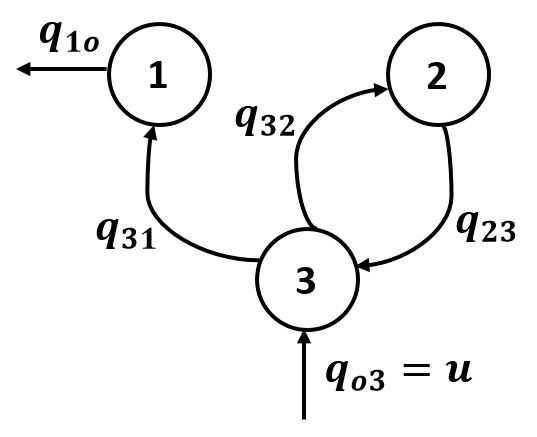
\includegraphics[width=0.3\textwidth]{graphe.JPG}
  \caption{}
  \label{graphe}
\end{figure}
 
 If we define the flux vector as
 \begin{equation}
 q(x,u)=
 \begin{bmatrix}
 q_{o3}(x,u)\\
 q_{10}(x,u)\\
 q_{23}(x,u)\\
 q_{31}(x,u)\\
 q_{32}(x,u)\\
 \end{bmatrix},
\label{eq:fluxvector}
\end{equation}
 the state-model can be written in a matrix format $\dot{x}=\mathbf{L}q(x,u)$, with
 \begin{equation}
 \mathbf{L}\triangleq
 \begin{pmatrix}
 0 & 1 & 0 & 1 & 0\\
 0 & 0 & 1 & 0 & -1\\
 1 & 0 & -1 & -1 & 1\\
 \end{pmatrix} .
\label{eq:L}
\end{equation}

The next step is to transform the system (\ref{eq:system}) into the form $\dot{x}=\mathbf{A}(x,u)x+\mathbf{B}u$. First of all, we have to know wether it makes sense or not. For this purpose, it must be proved that the multi-compartments model is a positive system. The flux vector $q(x,u)$ must fulfill some conditions :
\begin{itemize}
\item C1 : $q_{ij}(x,u)$ are positive functions on their domain.
\item C2 : $q_{ij}(x,u)$ are continuous and differentiable functions on their domain.
\item C3 : If $x_1 =0$, then $q_{ij}(x,u)=0$. No outflows for an empty compartment.
\end{itemize}

From the systems (\ref{eq:system}) and (\ref{eq:statemodel}), the $q_{ij}(x,u)$ functions can be deduced:
\begin{equation}
 q(x,u)=
 \begin{bmatrix}
 u\\
 \log(1+x_1)\\
x_2^2\\
x_3\\
x_3\\
 \end{bmatrix}.
\label{eq:qij}
\end{equation}
It is clear that the conditions are met. The system is positive and can be rewritten:
\begin{equation}
\begin{pmatrix}
\dot{x}_1\\
\dot{x}_2\\
\dot{x}_3\\
\end{pmatrix}=
\underbrace{
\begin{pmatrix}
-\dfrac{\log(1+x_1)}{x_1} & 0 & 1\\
0 & -x_2 & 1\\
0 & x_2 & -2\\
\end{pmatrix}}_{\mathbf{A}(x,u)}
\begin{pmatrix}
x_1\\
x_2\\
x_3\\
\end{pmatrix}+\underbrace{
\begin{pmatrix}
0\\
0\\
1\\
\end{pmatrix}}_{\mathbf{B}}u.
\label{eq:Ax}
\end{equation}
The matrix $\mathbf{A}(x,u)$ is a diagonally dominant Metzler matrix.

%%%%%%%EXO 4.2
\section*{4.2: An hydraulic system}
\begin{figure}[h!]
  \centering
  \includegraphics[width=0.4\textwidth]{systhydr}
  \caption{An hydraulic system}
  \label{syshydr}
\end{figure}

\subsection*{1)}
Given the hydraulic system shown in fig. \ref{syshydr}, we can deduce the following state model (considering volumetric flows $u_1=F_1$ and $u_2=F_2$ as input variables):
\begin{equation}
\left\{
  \begin{array}{l r}
  \dot{x}_1=u_1-q_{12}+u_2 &\\
  \dot{x}_2=q_{12}-q_{23}-q_{2o} & \textnormal{with } q_{ij}(x_i)=\dfrac{k_{ij}x_i\sqrt{x_i}}{S_i\beta_{ij}+x_i} \textnormal{ and } k_{ij}\triangleq\dfrac{\alpha_{ij}}{S_i}.~(\alpha_{ij},\beta_{ij}>0).\\
  \dot{x}_3=q_{23}-u_2 &\\
  \end{array} \right.
\label{eq:statemod}
\end{equation}
We observe that this state model {\it cannot} represent a compartmental system respecting C1-C3 conditions.
Indeed, the flow $q_{31} = u_2=F_2$ does not respect the C3 condition and the system is not positive:
\begin{itemize}
\item if $x_1=0$, $\dot{x}_1=F_1+F_2\geq 0$.
\item if $x_2=0$, $\dot{x}_2=q_{12}\geq 0$.
\item if $x_3=0$, the sign of $\dot{x}_3=q_{23}-F_2$ is undetermined.
\end{itemize}
If $x_3 =0$, that is to say the third compartment is empty, the model as stated still allows to pump water in the first vessel which can lead to negative vessels levels.

\subsection*{2)}
To ensure the system to be positive, the flow $q_{31}$ (which is the pumped flow $F_2$) has to be redefined such that it respects the physical reality and the C3 condition. This can be achieved as follows:
\begin{equation}
q_{31}(x_3,u_2) = \phi(x_3)u_2,
\label{eq:q31}
\end{equation}
where $\phi(x_3)$ is a positive function satisfying $\phi(0) = 0$ and $u_2$ represents the pump activation.

\subsection*{3)}
The state model can be rewritten as:
\begin{equation}
\left\{
  \begin{array}{l}
  \dot{x}_1=u_1-q_{12}+\phi(x_3)u_2\\
  \dot{x}_2=q_{12}-q_{23}-q_{2o}\\
  \dot{x}_3=q_{23}-\phi(x_3)u_2\\
  \end{array} \right.,
\label{eq:statemod2}
\end{equation}
and the associated graph is shown in fig. \ref{graph2}.\\

\begin{figure}[h!]
  \centering
  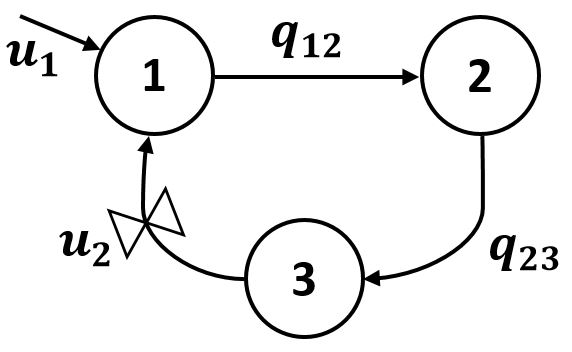
\includegraphics[width=0.3\textwidth]{graph2}
  \caption{}
  \label{graph2}
\end{figure}


%%%%%%EXO 4.3
\section*{4.3: A mixing vessels network}
\begin{figure}[h!]
  \centering
  \includegraphics[width=0.5\textwidth]{cuvmel}
  \caption{Mixing vessels network}
  \label{cuvmel}
\end{figure}
\subsection*{1)}
Given the system shown in fig. \ref{cuvmel}, we can set the state variables to be the volumes $V_{1,2}$ of the vessels and $x_{ij}$ corresponding to the amount of substance $i$ in the vessel of volume $V_j$ (thus $i=1..3$ and $j=1..2$, $x_{31}=0$). Using the inputs imposed by the wording, we obtain:
\begin{equation}
\begin{array}{l l}
\left\{
  \begin{array}{r c l}
  \dot{V}_1&=&F_1+F_2-u_1V_1\\
  \dot{V}_2&=&Q_1+F_3-u_2V_2\\
  \dot{x}_{11}&=&F_1u_3- x_{11}u_1\\
  \dot{x}_{21}&=&F_2u_4-x_{21}u_1 \\ 
  \dot{x}_{12}&=&x_{11}u_1-x_{12}u_2\\
  \dot{x}_{22}&=&x_{21}u_1-x_{22}u_2 \\
  \dot{x}_{32}&=&F_3u_5-x_{32}u_2 \\
  \end{array} \right.
  & \textnormal{with } u_1=\dfrac{Q_1}{V_1},~u_2=\dfrac{U_2}{V_2},~u_3=C_3,~u_4=C_4\textnormal{ and }u_5=C_3.\\
  \end{array}
\label{eq:statemodel3}
\end{equation}

\subsection*{2)}
The input variables form $u_1$ and $u_2$ allows the state model to be relevant even if the vessels are empty (condition C3). Indeed, we can see in the equations that:
\[
\textnormal{if }V_j=0\textnormal{, then }\dot{V}_j\geq 0 \textnormal{ as the term } -u_jV_j \textnormal{ is canceled.}
\]
It would not have been the same if the flows $Q_1$ and $Q_2$ were used as input variables.

%%%%%EXO 4.4
\section*{4.4: Compartments linear model}

\subsection*{1) Bidiagonal matrix}
Examples of (lower and upper) bidiagonal matrices for a 3-compartments model are shown below. In the first example, we can see that the quantity in the compartment $i$ is flowing to the compartment $i+1$. For the upper bidiagonal matrix, it is the opposite direction: $i \rightarrow i-1$. The associated graphs are presented in fig. \ref{fig:bidiagonal}.\\

\begin{minipage}[l]{0.55\linewidth}
	%\centering
	Examples: $
	\mathbf{A}=\begin{pmatrix}
	-1 & 0 & 0\\
	1 & -1 & 0\\
	0 & 1 & -1\\
	\end{pmatrix}$ or 
	$\begin{pmatrix}
	-1 & 1 & 0\\
	0 & -1 & 1\\
	0 & 0 & -1\\
	\end{pmatrix}$.
\end{minipage}
\begin{minipage}[r]{0.4\textwidth}
	\centering
	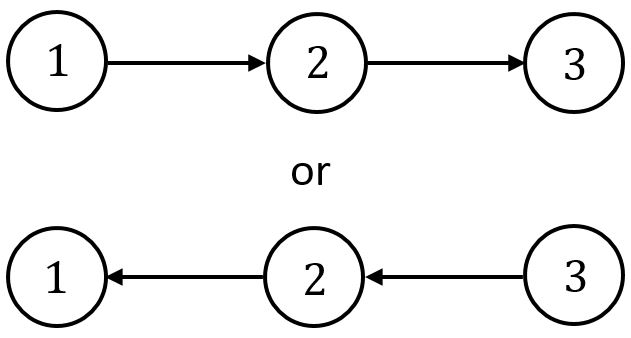
\includegraphics[width=0.6\textwidth]{bidiag}
	\captionof{figure}{}
	\label{fig:bidiagonal}
\end{minipage}

\subsection*{2) Tridiagonal matrix}
An example of a tridiagonal matrix for a 4-compartments model is shown below. Some elements are equals to $-2$ because $\mathbf{A}$ has to be a diagonally dominant Metzler matrix. Each vessel $i$ flows in the previous compartment $i-1$ and in the next one $i+1$ (except for the first and the last). The associated graph is presented in fig. \ref{fig:tridiagonal}.\\

\begin{minipage}[l]{0.5\linewidth}
	%\centering
	Example: $
	\mathbf{A}=\begin{pmatrix}
	-1 & 1 & 0 & 0\\
	1 & -2 & 1 & 0\\
	0 & 1 & -2 & 1\\
	0 & 0 & 1 & -1\\
	\end{pmatrix}$.
\end{minipage}
\begin{minipage}[r]{0.5\textwidth}
	\centering
	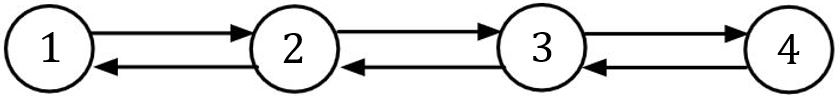
\includegraphics[width=0.8\textwidth]{tridiag}
	\captionof{figure}{}
	\label{fig:tridiagonal}
\end{minipage}

\subsection*{3) Lower tridiagonal matrix}
An example of a lower triangular matrix for a 4-compartments model is shown below. Each vessel $i$ flows in the next vessels $j$ ($j=i+1\rightarrow N$). The associated graph is presented in fig. \ref{fig:lowertri}.\\

\begin{minipage}[l]{0.5\linewidth}
	%\centering
	Example: $
	\mathbf{A}=\begin{pmatrix}
	-3 & 0 & 0 & 0\\
	1 & -2 & 0 & 0\\
	1 & 1 & -1 & 0\\
	1 & 1 & 1 & -1\\
	\end{pmatrix}$.
\end{minipage}
\begin{minipage}[r]{0.5\textwidth}
	\centering
	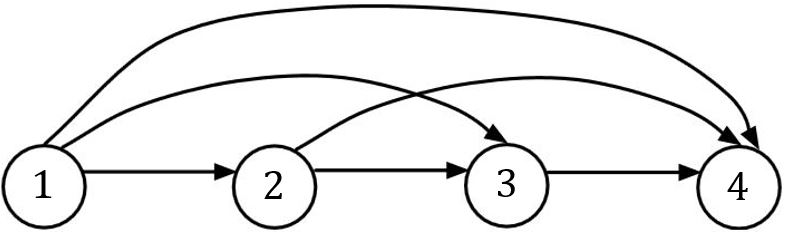
\includegraphics[width=0.8\textwidth]{lowertri}
	\captionof{figure}{}
	\label{fig:lowertri}
\end{minipage}

%%%%%EXO 4.5
\section*{4.5: Distillation process model}
From the example 4.13 presented in the course syllabus, the following state equations are obtained:
\begin{equation*} \begin{split}
\dot x_1 &= u_2 k(x_2) - u_{1}\frac{x_1}{m_1} - (u_2 - u_1) \frac{x_1}{m_1}\\
\dot x_2 &= u_1\frac{x_1}{m_1} - (u_1+u_3)\frac{x_2}{m_2} + u_2(k(x_3) - k(x_2)) + u_3c_f\\
\dot x_3 &= (u_1 + u_3)(\frac{x_2}{m_2} - \frac{x_3}{m_3}) + u_2(-\frac{x_3}{m_3} - k(x_3))
\end{split}. \end{equation*}

It can be rewritten under the form:
\begin{equation}
\begin{pmatrix}
\dot{x}_1\\
\dot{x}_2\\
\dot{x}_3\\
\end{pmatrix}=
\underbrace{
\begin{pmatrix}
-\frac{u_2}{m_1} & \frac{u_2k(x_2)}{x_2} & 0\\
\frac{u_1}{m_1}  & -\frac{(u_1+u_3)}{m_2}-\frac{u_2k(x_2)}{x_2}   & \frac{u_2k(x_3)}{x_3} \\
0 & \frac{(u_1+u_3)}{m_2} & -\frac{(u_2+u_3)}{m_3}-\frac{u_2k(x_3)}{x_3}\\
\end{pmatrix}}_{\mathbf{A}(x,u)}
\begin{pmatrix}
x_1\\
x_2\\
x_3\\
\end{pmatrix}+\underbrace{
\begin{pmatrix}
0\\
0\\
c_f\\
\end{pmatrix}}_{\mathbf{B}}
\begin{pmatrix}
u_1\\
u_2\\
u_3\\
\end{pmatrix}.
\label{eq:Ax5}
\end{equation}
The matrix $\mathbf{A}(x,u)$ is a diagonally dominant Metzler matrix as a physical condition gives $u_1<u_2$.

%%%%%EXO4.6
\section*{4.6: Communicating vessels}
\begin{figure}[h!]
  \centering
  \includegraphics[width=0.5\textwidth]{reservoircom}
  \caption{Communicating vessels}
  \label{reservoircom}
\end{figure}

\subsection*{1)}
Let $x_1$ and $x_2$ be set to the volumes contained in the vessel $1$ and $2$. Due to the physical nature of the problem, the second vessel cannot be more filled than the first one. Indeed, the fluid enters the system in the first vessel (the input variable is the input flow $u_1$) and flows out from the second vessel (output flow $q_{2o}$). In addition, the flow between the two vessels will be from the one with the highest water height to the one with the lower water height.\\

In a simplified case, the flow between two non communicating vessels $i$ and $j$ is given by the Torricelli's law:
\begin{equation}
q_{ij}=\dfrac{\alpha_{ij}h_i\sqrt{h_i}}{\beta_{ij}+h_i}.
\label{eq:torricelli}
\end{equation}
This law assumes that the output pressure is equal to the pressure at the top of the tank (atmospheric pressure). In our case, as the vessels are interconnected and the flow enters the second vessel at its base, we have to take into account the additional output pressure caused by a potential water column in the second vessel. The flow becomes:
\begin{equation}
	\begin{array}{r c l}
	q_{ij} &=& \dfrac{\alpha_{ij}(h_i-h_j)\sqrt{h_i-h_j}}{\beta_{ij}+(h_i-h_j)}\\
	& & \\
	          &=& \dfrac{\alpha_{ij}\Big(\dfrac{x_i}{S_i}-\dfrac{x_j}{S_j}\Big)\sqrt{\dfrac{x_i}{S_i}-\dfrac{x_j}{S_j}}}{\beta_{ij}+\Big(\dfrac{x_i}{S_i}-\dfrac{x_j}{S_j}\Big)}\\
	  \end{array}.
\label{eq:torricellimod}
\end{equation}

The flows can be expressed as:
\begin{equation}
	\begin{array}{r c l}         
	 q_{12} &=&\dfrac{\alpha_{12}\Big(\dfrac{x_1}{S_1}-\dfrac{x_2}{S_2}\Big)\sqrt{\dfrac{x_1}{S_1}-\dfrac{x_2}{S_2}}}{\beta_{12}+\Big(\dfrac{x_1}{S_1}-\dfrac{x_2}{S_2}\Big)} \\
	 q_{2o}&=&\dfrac{k_{2o}x_2\sqrt{x_2}}{S_2\beta_{2o}+x_2}\\
	\end{array}.
\label{eq:flow6}
\end{equation}

The system state model can now be established.
\begin{equation}
\left\{
  \begin{array}{l}
  \dot{x}_1=u_1-\dfrac{\alpha_{12}\dfrac{x_1}{S_1}\sqrt{\dfrac{x_1}{S_1}-\dfrac{x_2}{S_2}}}{\beta_{12}+\Big(\dfrac{x_1}{S_1}-\dfrac{x_2}{S_2}\Big)}+\dfrac{\alpha_{12}\dfrac{x_2}{S_2}\sqrt{\dfrac{x_1}{S_1}-\dfrac{x_2}{S_2}}}{\beta_{12}+\Big(\dfrac{x_1}{S_1}-\dfrac{x_2}{S_2}\Big)} \\
  \\
  \dot{x}_2=\dfrac{\alpha_{12}\dfrac{x_1}{S_1}\sqrt{\dfrac{x_1}{S_1}-\dfrac{x_2}{S_2}}}{\beta_{12}+\Big(\dfrac{x_1}{S_1}-\dfrac{x_2}{S_2}\Big)}-\dfrac{\alpha_{12}\dfrac{x_2}{S_2}\sqrt{\dfrac{x_1}{S_1}-\dfrac{x_2}{S_2}}}{\beta_{12}+\Big(\dfrac{x_1}{S_1}-\dfrac{x_2}{S_2}\Big)}-\dfrac{k_{2o}x_2\sqrt{x_2}}{S_2\beta_{2o}+x_2}\\
  \end{array} \right..
\label{eq:statemod6}
\end{equation}

\subsection*{2)}
From the flows expressions found in equation (\ref{eq:flow6}), we are able to see directly that the conditions $C_1$ and $C_2$ are met as we have the physical condition $h_1=x_1/S_1 \geq h_2 = x_2/S_2$. If we look closely to the state model (\ref{eq:statemod6}), it appears that:
\begin{itemize}
\item If $x_1=0$, then $x_2 =0$ and $\dot{x}_1=u_1\geq 0$.
\item If $x_2=0$ then $\dot{x}_2=\dfrac{\alpha_{12}\dfrac{x_1}{S_1}\sqrt{\dfrac{x_1}{S_1}}}{\beta_{12}+\dfrac{x_1}{S_1}}\geq 0$.
\end{itemize}
The condition $C_3$ is also respected. The associated graph is shown in fig. \ref{graph6}.\\

\begin{figure}[h!]
  \centering
  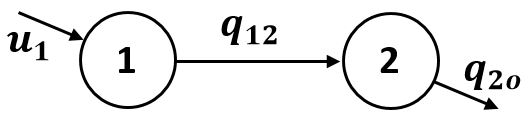
\includegraphics[width=0.3\textwidth]{graph6}
  \caption{}
  \label{graph6}
\end{figure}
